\documentclass[a6paper,11pt,english]{article}

\usepackage[margin=0.25in]{geometry}

\usepackage{amsmath}

\usepackage[ngerman]{babel}
\usepackage[utf8]{inputenc}
\usepackage[babel,german=quotes]{csquotes}
\usepackage[hyphens]{url}
\usepackage{listings}
\usepackage{color}
\usepackage{textcomp}
\usepackage[breaklinks]{hyperref}
\usepackage{framed} 
\usepackage[ngerman]{translator}
\usepackage{setspace}
\usepackage{graphicx}


% Sans-Serif-Font
\renewcommand{\familydefault}{\sfdefault}

% kein Einzug in erster Zeile
\setlength{\parindent}{0pt}

% dafür etwas Abstand
\setlength{\parskip}{5pt}

\makeatletter
\DeclareRobustCommand{\em}{%
  \@nomath\em \if b\expandafter\@car\f@series\@nil
  \normalfont \else \bfseries \fi}
\makeatother

% infobox
\definecolor{boxBG}{rgb}{0.90,0.90,0.96}
\makeatletter\newenvironment{infobox}{%
   \begin{lrbox}{\@tempboxa}\begin{minipage}{\columnwidth}\footnotesize \emph{INFO:} }{\end{minipage}\end{lrbox}%
   \colorbox{boxBG}{\hspace{0pt}\usebox{\@tempboxa}\hspace{0pt}}
}\makeatother

% Additional Options
\definecolor{javared}{rgb}{0.6,0,0} % for strings
\definecolor{javagreen}{rgb}{0.25,0.5,0.35} % comments
\definecolor{javapurple}{rgb}{0.5,0,0.35} % keywords
\definecolor{javadocblue}{rgb}{0.25,0.35,0.75} % javadoc
\definecolor{grey}{rgb}{0.75,0.75,0.75}
\definecolor{darkgrey}{rgb}{0.3,0.3,0.3}
\definecolor{lightgrey}{rgb}{0.95,0.95,0.95}
\definecolor{listingbg}{rgb}{0.90,0.96,0.90}

\lstset{
	language=Python,
	basicstyle=\ttfamily,
	keywordstyle=\color{javapurple}\bfseries,
	stringstyle=\color{javared},
	commentstyle=\color{javagreen},
	morecomment=[s][\color{javadocblue}]{/**}{*/},
	numbers=none,
	numberstyle=\color{darkgrey},
	stepnumber=1,
	numbersep=10pt,
	tabsize=4,
	showspaces=false,
	showstringspaces=false,
	breaklines=true,
	breakatwhitespace=false,
	prebreak = \raisebox{0ex}[0ex][0ex]{\ensuremath{\hookleftarrow}},
	frame=l,
	rulecolor=\color{javagreen},
	columns=flexible,
	backgroundcolor=\color{listingbg},
	inputencoding=utf8,
	extendedchars=true,
	literate={Ö}{{\"O}}1 {Ä}{{\"A}}1 {Ü}{{\"U}}1 {ß}{{\ss}}2 {ü}{{\"u}}1 {ä}{{\"a}}1 {ö}{{\"o}}1 {µ}{\textmu}1
}

\hypersetup{
	pdfborder=0 0 0,
	pdffitwindow=false,    % window fit to page when opened
	pdfstartview={FitH}    % fits the width of the page to the window  
}
\include{glossary}

\begin{document}
	\begin{center}
		\section*{\enquote{Variablen}}
		\section*{Wie merke ich mir einen Wert?}	
	\end{center}
	
	
	\begin{figure}[htbp]
		\centering
		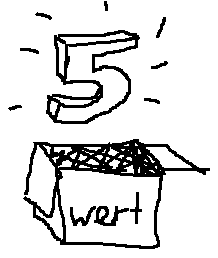
\includegraphics[width=0.9\textwidth]{img/variablen.png}
		\label{variablen}
	\end{figure}
	
	
	\newpage
	
	\begin{lstlisting}
# 5 unter dem Namen "meinWert" merken
meinWert = 5

# "meinWert" ausgeben
print(meinWert) # 5

# "meinWert" verdoppeln
meinWert = meinWert * 2
print(meinWert) # 10

# mit Variablen Rechnen:
zweiterWert = 2
ergebnis = meinwert + zweiterWert # 10 + 2
print(ergebnis) # 12

# geht auch mit Zeichenketten:
meinWert = "Hallo"
zweiterWert = "Welt!"
print(meinWert) # Hallo
print(zweiterWert) # Welt!
print(meinWert + "..." + zweiterWert) # Hallo...Welt!

# Wert einer Variablen in einer anderen Variablen speichern:
hallo = meinWert
print(meinWert) # Hallo
print(hallo)  # Hallo
	\end{lstlisting}
	
	
	
\end{document}